\section{Track 2: Color Analysis}
Within the bicycle distribution industry, the base color attribute acts as a useful dealer order signal reflecting localized predictions of end-consumer preferences by dealers. Table \ref{tab:color} and Figure \ref{fig:color} illustrate the Top 10 primary colors dominating the upcoming procurement cycle.

\subsection{Color Contribution and Inventory Implications}
Top colors listed below serve as strong candidates for procurement assurance, heavily driving the bulk of inventory planning. Conversely, low or declining colors require an inventory watch to mitigate stagnant stock. It is crucial to note that this color forecast exclusively reflects a dealer order signal, and should not be perfectly conflated with absolute end-consumer preference.

\begin{table}[H]
\centering
\small
\caption{Top Color Contribution Summary}
\label{tab:color}
\resizebox{\linewidth}{!}{
\begin{tabular}{lllll}
\toprule
\textbf{Color} & \textbf{Forecast Qty} & \textbf{Qty Share} & \textbf{Forecast Rev (VND)} & \textbf{Rev Share} \\
\midrule
Cream & 6,549 & 17.4\% & 10,178,738,540 & 16.7\% \\
Black & 5,797 & 15.4\% & 10,170,423,274 & 16.7\% \\
Gray & 4,308 & 11.5\% & 8,112,828,292 & 13.3\% \\
Pink & 3,816 & 10.1\% & 5,486,401,943 & 9.0\% \\
Green & 3,253 & 8.7\% & 5,418,630,863 & 8.9\% \\
Blue & 3,136 & 8.3\% & 4,786,143,217 & 7.9\% \\
White & 2,857 & 7.6\% & 4,997,821,606 & 8.2\% \\
Brown & 2,018 & 5.4\% & 3,055,462,552 & 5.0\% \\
Mint & 1,968 & 5.2\% & 3,005,926,217 & 4.9\% \\
Red & 1,707 & 4.5\% & 2,520,059,229 & 4.1\% \\
\bottomrule
\end{tabular}
}
\begin{flushleft}
\footnotesize \textit{Note.} Source: outputs/modeling/phase3\_color\_summary\_q2\_2026.csv (columns: Group\_Share\_Base\_Qty, Group\_Share\_Base\_Rev). Forecast revenue is computed from the Group-Share proportional allocation applied to each base color. Qty Share and Rev Share are computed as a percentage of the total Q2 Base scenario forecast (37,596 units / 60,914,780,907 VND).
\end{flushleft}
\end{table}


\begin{figure}[H]
\centering
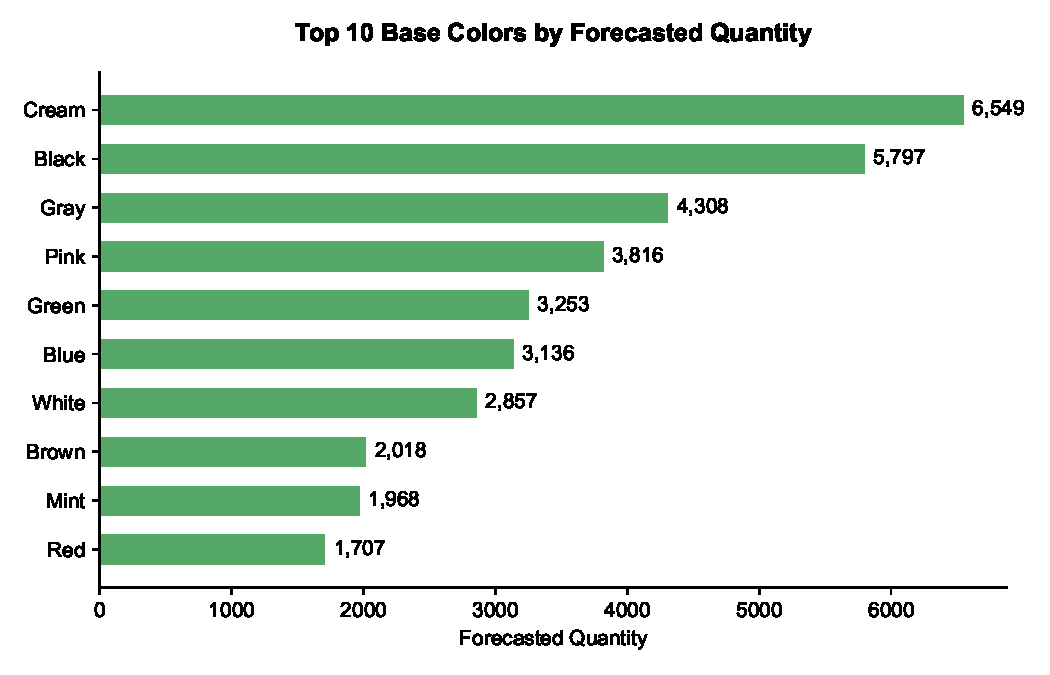
\includegraphics[width=0.85\textwidth]{../figures/en/color_summary.pdf}
\caption{Top 10 Base Colors by Forecasted Quantity (Base Scenario)}
\label{fig:color}
\end{figure}

Colors falling outside this Top 10 tier, or those exhibiting severe historical demand slumps, are systematically flagged as slow-moving SKUs. This automated flagging empowers the sales department to execute early inventory liquidations, phasing out unviable variants before they negatively impact warehouse capacity.
\FloatBarrier
